\PassOptionsToPackage{hyperfootnotes=false}{hyperref}
\documentclass{beamer}
\usefonttheme{professionalfonts}
%\usetheme{Rochester}
%\usetheme{AnnArbor}
\usetheme{Szeged}
\useoutertheme{infolines}
\usecolortheme{dolphin}
\usepackage{graphicx}
% \usepackage[english]{babel}
\usepackage{multicol}
\usepackage{color}
\usepackage{xcolor}
%\usepackage{smartdiagram}


%\definecolor{carmine}{rgb}{0.59, 0.0, 0.09}
\usepackage{amsmath} 

\usepackage{graphicx}
\usepackage{tikz}
\usetikzlibrary{shapes.callouts}
\usepackage{multirow}

\usepackage[utf8]{inputenc}

\usepackage{enumerate}
\usepackage[shortlabels]{enumitem}
\usepackage{amsmath,amsthm,amssymb,amsfonts,mathrsfs,latexsym,stmaryrd}
\usepackage{tcolorbox}

\usepackage{color} 
\usepackage{amssymb, amsmath, amsbsy}
\usepackage{adjustbox,lipsum}
\usepackage{placeins}

\usepackage{textpos}
\usepackage{wrapfig}
\usepackage[spanish, es-tabla]{babel}

\usepackage{caption}
\setlength{\parindent}{0pt}

\usepackage{url}
\usepackage{float}
\usepackage{tikz}
\usetikzlibrary{patterns}


\title[ICS-162]{Econometría ICS-294\\ \small{Clase 20: Series de tiempo}}

\author{Jocelyn Tapia Stefanon}
\institute[USM]
{Universidad Técnica Federico Santa María\\ % Your institution for the title page
	\medskip
	\textit{} % Your email address
	
}
\logo{

\includegraphics[width=1cm]{Logo.png}
}
\date{}
\newcommand\Fontvi{\fontsize{9}{7.2}\selectfont}
\begin{document}


\frame{\titlepage}



\begin{frame}{¿Qué es una Serie de Tiempo?}
Una \textbf{serie de tiempo} es un conjunto de observaciones cuantitativas ordenadas cronológicamente:
\[
Y_1, Y_2, ..., Y_T
\]
donde $Y_t$ es el valor observado en el instante $t$.

Las series de tiempo pueden presentar:
\begin{itemize}
    \item Tendencia
    \item Ciclos
    \item Estacionalidad
    \item Aleatoriedad
\end{itemize}
\end{frame}

\begin{frame}{Tipos de Modelos}
\begin{block}{Modelos deterministas}
Métodos simples de extrapolación sin considerar aleatoriedad. Ejemplo: promedio móvil.
\end{block}

\begin{block}{Modelos estocásticos}
Describen procesos aleatorios subyacentes usando variables aleatorias y distribuciones.
\end{block}
\end{frame}

% \begin{frame}{Estacionariedad}
% \textbf{Serie estacionaria:}
% \begin{itemize}
%     \item Media constante: $\mathbb{E}(Y_t) = \mathbb{E}(Y_{t+m})$
%     \item Varianza constante: $\text{Var}(Y_t) = \text{Var}(Y_{t+m})$
%     \item Covarianza depende solo del rezago: $\text{Cov}(Y_t, Y_{t+k}) = \text{Cov}(Y_{t+m}, Y_{t+m+k})$
% \end{itemize}

% \textbf{Serie no estacionaria:} sus características cambian con el tiempo. Puede hacerse estacionaria mediante diferenciación.
% \end{frame}

\begin{frame}{Componentes Clásicos de una Serie}
\begin{itemize}
    \item Tendencia ($T$): evolución a largo plazo.
    \item Ciclo ($C$): fluctuaciones de largo plazo no periódicas.
    \item Estacionalidad ($E$): variaciones periódicas de corto plazo.
    \item Aleatoriedad ($A$): componente residual, ruido.
\end{itemize}

\textbf{Modelos comunes:}
\begin{itemize}
    \item Aditivo: $Y(t) = T(t) + C(t) + E(t) + A(t)$
    \item Multiplicativo: $Y(t) = T(t) \cdot C(t) \cdot E(t) \cdot A(t)$
\end{itemize}
\end{frame}

\begin{frame}{Componentes}
\begin{figure}
    \centering
    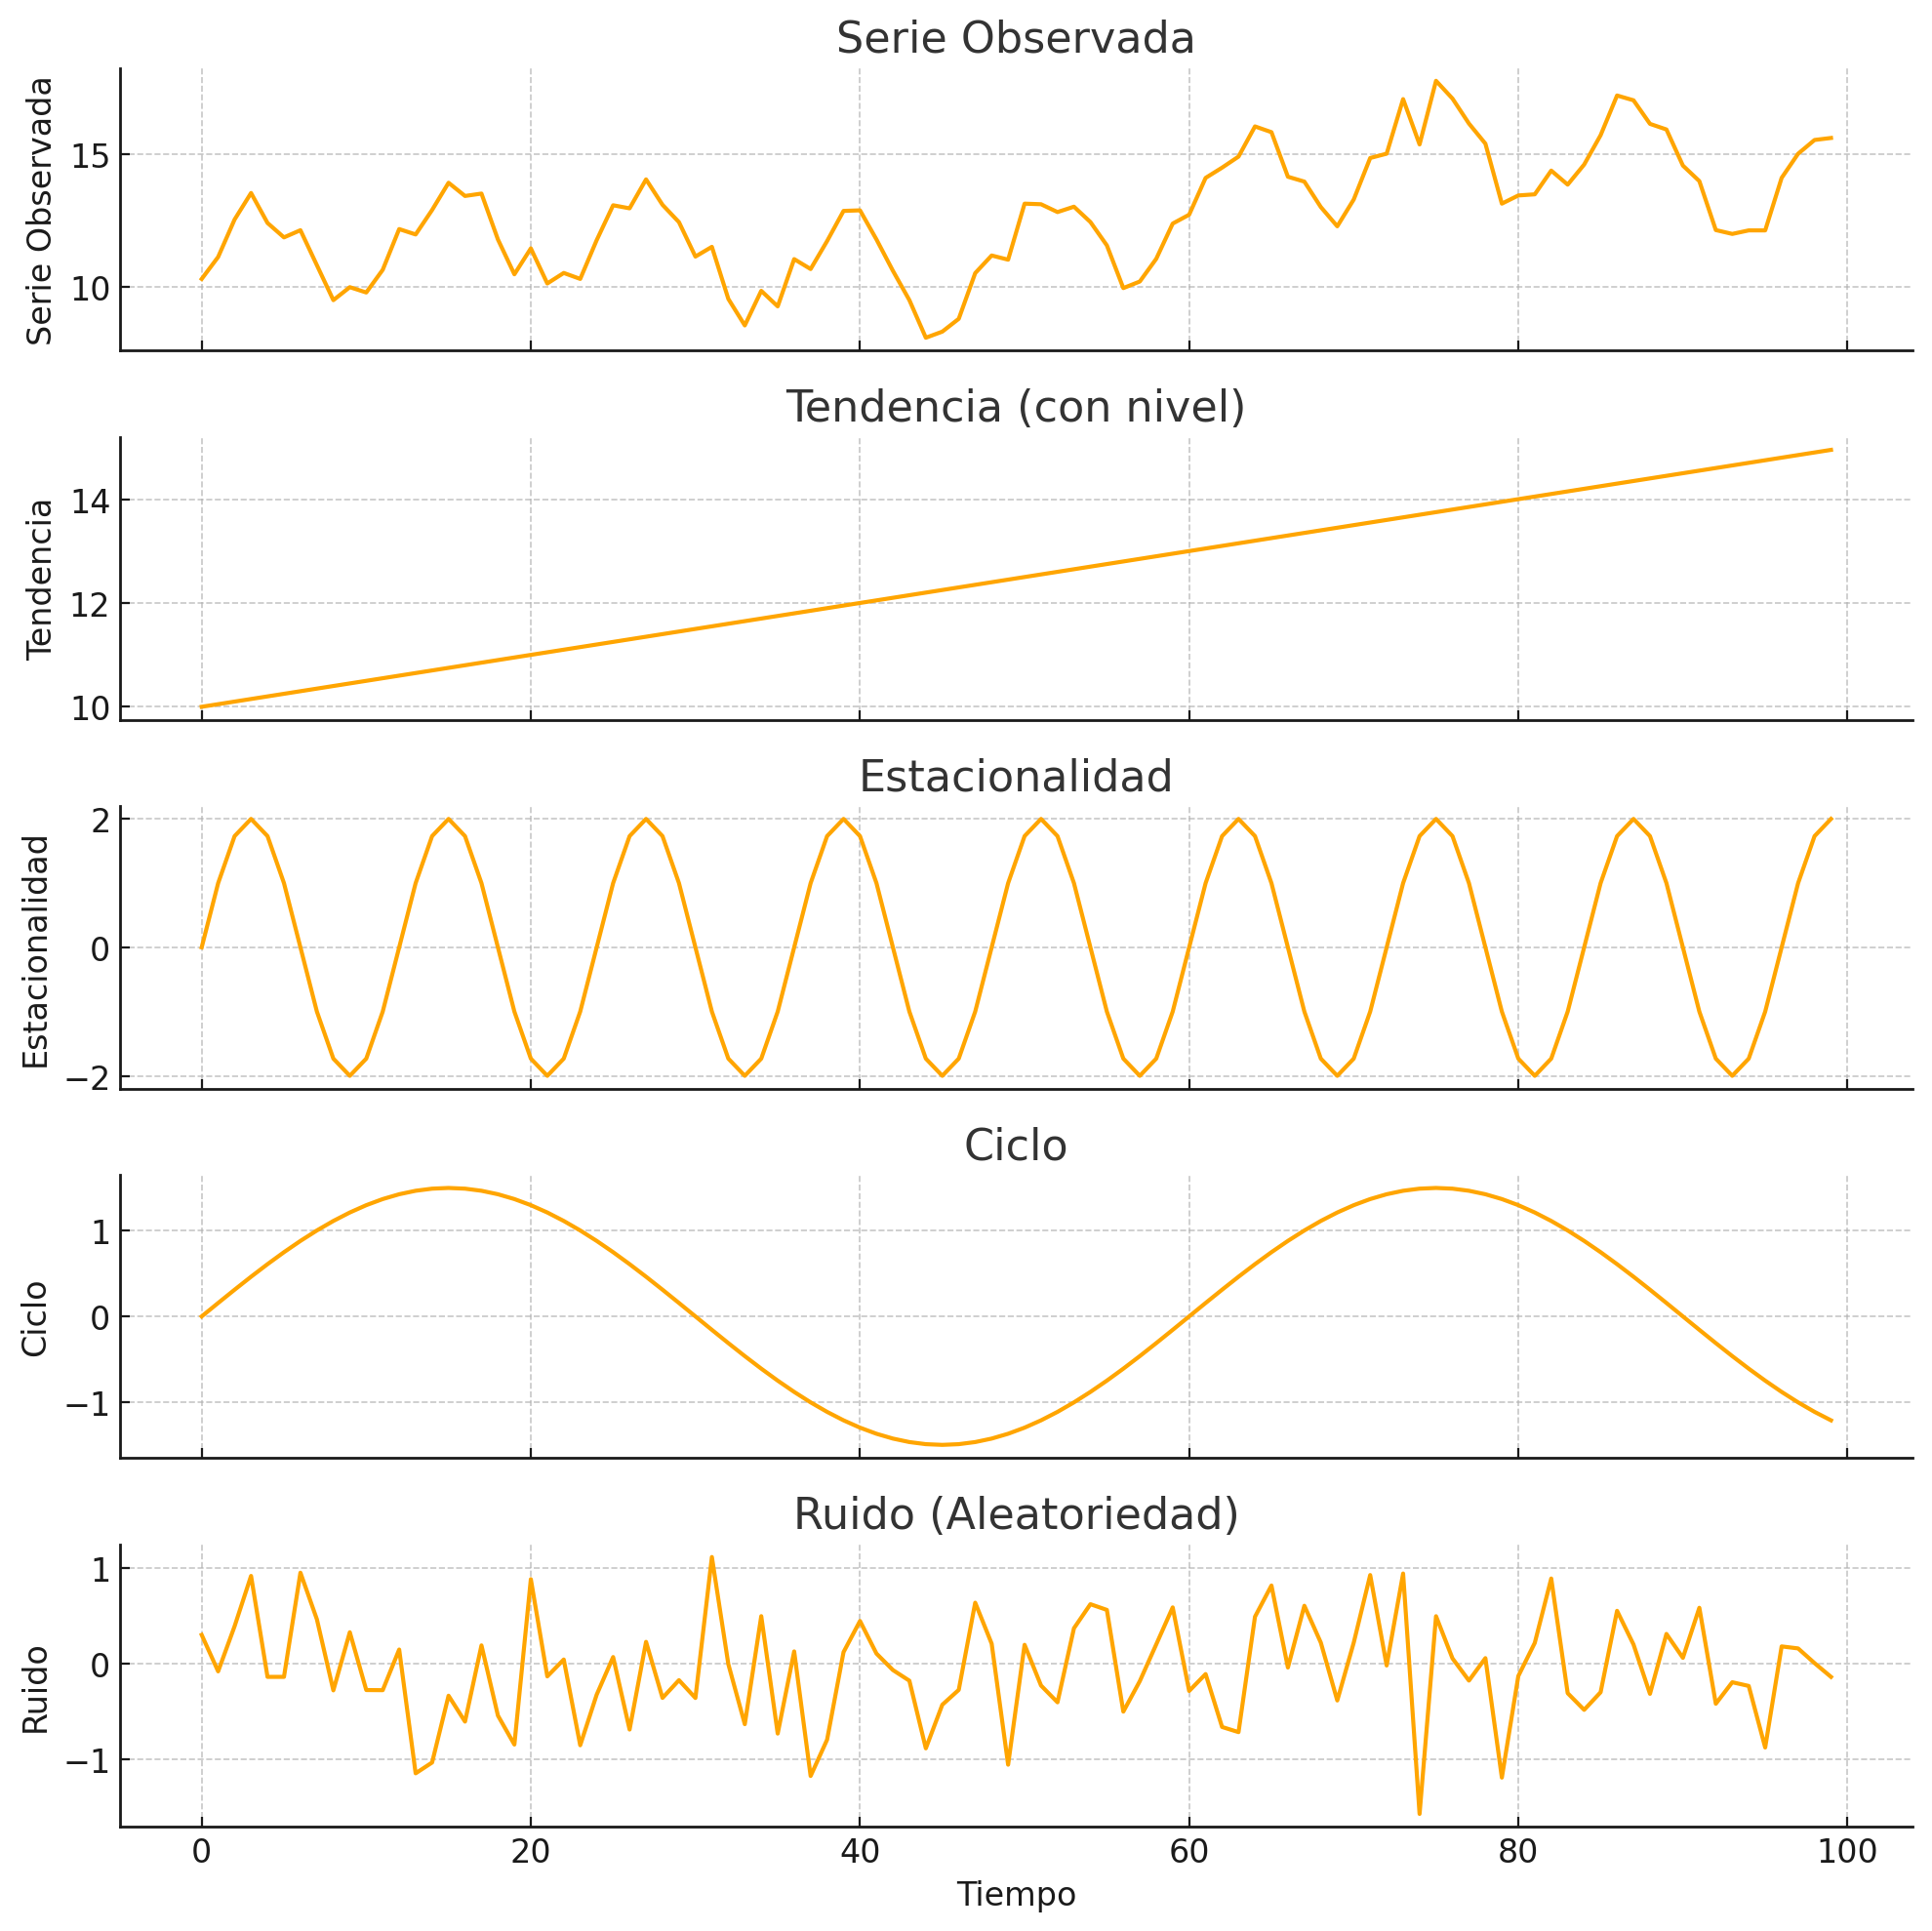
\includegraphics[width=0.65\linewidth]{images/descomposicion_serie.png}
\end{figure}
\end{frame}

\begin{frame}
\frametitle{Ejemplo: Ventas Mensuales de Helados}

\begin{itemize}
    \item \textbf{Tendencia (T)}: crecimiento anual de las ventas por aumento poblacional.
    \item \textbf{Ciclo (C)}: caídas temporales por recesiones o eventos globales.
    \item \textbf{Estacionalidad (E)}: ventas más altas en verano, más bajas en invierno.
    \item \textbf{Aleatoriedad (A)}: variaciones impredecibles (semanas muy calurosas fuera de temporada, cortes eléctricos, etc.).
\end{itemize}

\begin{figure}
    \centering
    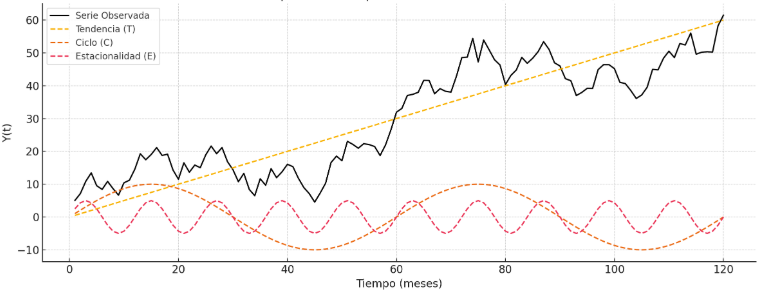
\includegraphics[width=0.75\linewidth]{images/venta_helado.png}
\end{figure}

\end{frame}

\begin{frame}
\frametitle{Proceso Estocástico}
\begin{itemize}
    \item Una serie de tiempo es una realización de un proceso estocástico: \(\{Y_t\}\)
    \item Un proceso estocástico es una colección de variables aleatorias indexadas por el tiempo.

    \[
\{ Y_t : t \in T \}
\]

donde \( T \) es el conjunto de tiempos (por ejemplo, \( T = \{1, 2, 3, \dots\} \) para datos discretos).

Cada \( Y_t \) es una variable aleatoria definida sobre un mismo espacio de probabilidad 
\((\Omega, \mathcal{F}, P)\), con una función de probabilidad conjunta que describe su comportamiento 
a lo largo del tiempo.

    \item Permite modelar la evolución temporal de fenómenos como precios, rendimientos, consumo, producción, etc.
\end{itemize}


\end{frame}

\begin{frame}{Proceso estocástico}
   \begin{itemize}
    \item \( \Omega \): representa el \textbf{espacio muestral}, es decir, el conjunto de todos los escenarios posibles del mundo 
    (todas las trayectorias que podrían ocurrir).

    \item \( \mathcal{F} \): es la \textbf{\(\sigma\)-álgebra} (sigma-álgebra), el conjunto de subconjuntos de \( \Omega \) sobre los cuales 
    se pueden definir eventos o sucesos medibles (por ejemplo: ``el PIB sube tres trimestres seguidos'').

    \item \( P \): es la \textbf{medida de probabilidad}, que asigna a cada evento \( A \in \mathcal{F} \) una probabilidad
    \( P(A) \in [0,1] \); en otras palabras, son las reglas del azar que gobiernan el proceso estocástico.
\end{itemize}

Así, cada variable \( Y_t \) es una función que asocia a cada escenario posible \( \omega \in \Omega \) 
un valor real \( Y_t(\omega) \), y la colección completa \( \{Y_t\} \) describe la evolución de esa variable a lo largo del tiempo.
 
\end{frame}

\begin{frame}{Ejemplo}
\small
\begin{itemize}
    \item Imaginemos que \( Y_t \) representa el \textbf{Producto Interno Bruto (PIB)} real trimestral de un país.
    
    \item El \emph{proceso estocástico} \( \{ Y_t : t \in T \} \) describe todas las posibles trayectorias 
    que el PIB podría seguir en distintos mundos posibles, es decir, bajo diferentes realizaciones 
    del azar \( \omega \in \Omega \).
    
    \item La \emph{serie de tiempo observada} corresponde a la trayectoria particular que efectivamente 
    ocurrió en nuestro mundo.
    
    \item En otras palabras, observamos una secuencia concreta de valores:
    \[
    y_t = Y_t(\omega_0), \quad t = 1, 2, \dots, T,
    \]
    para una realización específica \( \omega_0 \in \Omega \).
\end{itemize}
\end{frame}




\begin{frame}
\frametitle{Estacionariedad y Autocorrelación}
\begin{itemize}
   % \item Un proceso \(\{X_t\}\) es \textbf{estacionario en sentido estricto} si su distribución conjunta no cambia con el tiempo:
   % \[    (X_{t_1}, \ldots, X_{t_k}) \overset{d}{=} (X_{t_1+h}, \ldots, X_{t_k+h}) \quad \forall h \in \mathbb{Z} \]
    \item  Un proceso \(\{X_t\}\) es \textbf{estacionario } (débilmente o de segundo orden) si:
    \begin{itemize}
        \item Esperanza constante: \(\mathbb{E}[X_t] = \mu\)
        \item Varianza constante: \(\text{Var}(X_t) = \sigma^2 < \infty\)
        \item Covarianza depende solo del rezago: \(\gamma(h) = \text{Cov}(X_t, X_{t+h})\)
    \end{itemize}
    \item La \textbf{función de autocorrelación} es:
    \[
    \rho(h) = \frac{\gamma(h)}{\gamma(0)} = \frac{\text{Cov}(X_t, X_{t+h})}{\text{Var}(X_t)}
    \]
    \item En procesos estacionarios: \(\rho(h)\) depende solo del rezago \(h\), no del tiempo \(t\).
\end{itemize}
\end{frame}

\begin{frame}
\frametitle{Ruido Blanco}
\begin{itemize}
    \item Es un proceso estocástico \(\{\varepsilon_t\}\) con:
    \begin{itemize}
        \item Media cero: \(\mathbb{E}[\varepsilon_t] = 0\)
        \item Varianza constante: \(\text{Var}(\varepsilon_t) = \sigma^2\)
        \item No autocorrelación: \(\text{Cov}(\varepsilon_t, \varepsilon_{t+h}) = 0\) si \(h \neq 0\)
    \end{itemize}
    \item Es la base para construir modelos más complejos.
\end{itemize}
\end{frame}
\begin{frame}
\frametitle{Modelo Autorregresivo AR(p)}
\begin{itemize}
    \item Un modelo AR(p) se basa en los valores pasados de la serie:
    \[
    Y_t = \phi_1 Y_{t-1} + \cdots + \phi_p Y_{t-p} + \varepsilon_t \]

     Donde $\varepsilon_t$ es un ruido blanco.

    \item Ejemplo AR(1):
     \[
     Y_t = \phi Y_{t-1} + \varepsilon_t
     \]
\end{itemize}
 \end{frame}

\begin{frame}
\frametitle{Modelo de Media Móvil MA(q)}
\begin{itemize}
    \item El modelo MA(q) usa errores pasados:
    \[
    Y_t = \varepsilon_t + \theta_1 \varepsilon_{t-1} + \cdots + \theta_q \varepsilon_{t-q}
    \]
    \item Ejemplo MA(1):
    \[
    Y_t = \varepsilon_t + \theta \varepsilon_{t-1}
    \]
 \item Donde $\varepsilon_t$ es un ruido blanco.
\end{itemize}
\end{frame}


\begin{frame}{Correlograma }
    \begin{figure}
        \centering
        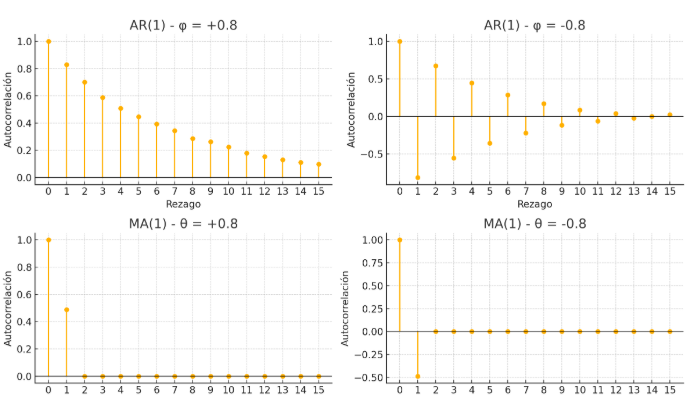
\includegraphics[width=0.85\linewidth]{images/correlograma1.png}
    \end{figure}
\end{frame}


\end{document}
